\chapter{Réalisation}
% l’ordre de présentation le plus logique est souvent l’ordre chronologique dans lequel les tâches ont été accomplies. Il faut présenter les points forts en distinguant nettement l’existant et la plus-value apportée par le stagiaire. Si des solutions ont été envisagées, mais non retenues, il peut être intéressant de les présenter en expliquant pourquoi elles ont été abandonnées. C’est toute la chaîne, de la prise de connaissance du problème à la solution apportée, qui doit être déroulée.

% Cette partie débouche nécessairement sur des résultats qu’il faut énoncer en précisant leurs exploitations actuelles ou à venir. Il faut annoncer clairement ce qui a été réalisé ou non par rapport à la mission de départ. Cette partie peut être complétée par des propositions personnelles du stagiaire pour prolonger son travail, et même par des critiques positives de son environnement de travail.

% Tentative plan
%5.1. recherche doc
%5.2. patch "reimplement"
%5.3. build "growing"
%5.4. optimise "growing"
%5.5. conclusions on "growing" and "awd"
%5.6. preparing "papud" \& basic model
%5.7. understanding strange comportment \& preparing corpus
%5.8. conclusions on "papud"

\section{\Glsentrytext{project_gmsnn}} % TODO nommer ce projet
\subsection{Recherche documentaire}
La première partie du projet, qui à durée à peu près une semaine, à été la recherche documentaire et la prise en main des outils.
Ce travail à été effectué à partir des documents fournis par notre maître de stage, de la documentation de \gls{pytorch}\autocite{60MinBlitzTorch,ByExampleTorch,Classify,doc_pytorch} et de \gls{g5k}, complétés par nos recherches personnelles.
%TODO cite articles fournis
%TODO cite g5k doc
%TODO cite recherches personnelle

%-> liste de ref bib % lib, tutos, concepts
\subsection{Étude et ré-implémentation simplifiée du modèle \gls{soa}}
\subsubsection{Travail effectué}
La deuxième partie du projet à été la prise en main de la base de code fournie.
Il s'agit d'une implémentation \gls{soa} d'un \gls{lm} au niveau du caractère, sur laquelle notre maître de stage avait commencé à travailler.
Le code d'origine provient du dépôt \og awd-lstm-lm\fg{}\autocite{awd_source}, qui contenait un modèle \gls{soa} de \gls{lm} au niveau du caractère.

Au début du stage, la base de code contenait~:
\begin{itemize}
	\item la version d'origine du dépôt~;
	\item un début de ré-implémentation simplifiée du \gls{model} de la version d'origine~; cette version  devait servir de base pour développer le \gls{model} du \gls{gmsnn}, ainsi que de comparaison pour les performances du nouveau \gls{model}~; elle comportait quelques \glspl{bug} et ne fonctionnait pas en l'état~;
	\item un début de travail sur l'architecture du \gls{gmsnn}.
\end{itemize}

\vspace{1em}
L'objectif de cette étape était de faire fonctionner la ré-implémentation simplifiée du \gls{model}.

Pour cela, nous avons déchiffré et re-documenté le code, qui contenait des fragments obsolètes et peu documentés.
Après le déchiffrage, il à fallu comprendre et réparer les fragments défectueux.

\newpage
\subsubsection[\Glsentrytext{model} ré-implémenté simplifiée]{\Gls{model} ré-implémenté simplifiée}
Le \gls{model} simplifiée produit est composé d'un module encodant les caractères, d'un \gls{rnn} particulier (un \gls{lstm}, voir \autoref{def:lstm}), et d'un module produisant une distribution de probabilité sur les caractères connus. La \autoref{fig:reimplement} représente cette architecture.

\begin{figure}[h]
	\centering
	\scalebox{1}{\usetikzlibrary{calc}
\newsavebox\mydictbox
\savebox\mydictbox{%
  
\includegraphics[width=3em]{/home/emarquer/InternshipSynalp2018/report_internship/images/tool_translate_offline_dictionary.png}
}

\begin{tikzpicture}[shorten >=2pt,->,draw=black, node distance=7em]
    \tikzstyle{every pin edge}=[<-,shorten <=2pt]
	\tikzstyle{module}=[minimum size=3em, fill=gray!50!]
	\tikzstyle{char}=[module, circle, fill=green!50!]%, label={below:\usebox\mydictbox}]
	\tikzstyle{text label}=[rectangle, text centered, text width=7em, node distance=5em]
	\tikzstyle{nn}=[rectangle, module, fill=orange!50!]
	\tikzstyle{rnn}=[nn, fill=red!50!]

	\node[char] (char) {\$};
	\node[nn, right of=char] (emb) {Emb.};
	\node[rnn, right of=emb] (rnn) {LSTM};
	\draw[->] (rnn.north) to [out=90,in=90, looseness=2] ($(rnn.west) + (-0.5,0)$) to [out=-90,in=-90, looseness=2] (rnn.south);
	\node[nn, right of=rnn] (lin) {Lin.};
	\node[char, right of=lin] (out) {P(\$$_{+1}$)};
	\draw[->] (char) to (emb);
	\draw[->] (emb) to (rnn);
	\draw[->] (rnn) to (lin);
	\draw[->] (lin) to (out);
	%\node[char] (char) {\$};


    \node[text label, above of=char] (charl) {Caract\`{e}re};
    \node[text label, above of=emb] (embl) {Encodage du caract\`{e}re};
    \node[text label, above of=rnn] (rnnl) {RNN};
    \node[text label, above of=lin] (linl) {Transformation en distribution de probabilit\'{e}};
    \node[text label, above of=out] (outl) {Probabilit\'{e} d'apparition des caract\`{e}res};
\end{tikzpicture}}
	\caption[Architecture du \glsentrytext{model} réimplémenté]{Architecture du \gls{model} réimplémenté. Le modèle prend en entrée des caractères, et produit des probabilités sur quel caractère apparaîtra ensuite.}\label{fig:reimplement}
\end{figure}

Le module d'encodage des caractères, appelé \foreign{embeding layer} en anglais (littéralement \og couche d'inclusion\fg{}), produit une représentation apprise de chaque caractère sous forme de \gls{tensor}. Ce \gls{tensor} est appelé \gls{embedding}. Ce module, entraîné, peut apprendre des propriétés spécifiques à chaque caractère. Par exemple ce module peut apprendre que telle lettre est une consonne et que telle autre est un caractère de ponctuation. \label{def:embeding}

Le \gls{rnn} traite les caractères sous forme de séquence, et peut ainsi apprendre la structure en mots, la syntaxe et d'autres propriétés du langage.

Le module produisant la distribution de probabilité est un module linéaire.
Il transforme les informations produites par le réseau de neurones en probabilité pour chaque caractère d'être le prochain caractère de la séquence. % TODO def module linéaire

Voir les annexes \ref{subsec:testreimp_1}, \ref{subsec:testreimp_2} et \ref{subsec:testreimp_3} pour les rapports sur le \gls{model} ré-implémenté. 

\subsubsection{Conclusion}
Cette étape, outre la préparation du code, à permit la mise en œuvre et une meilleur compréhension des concepts appris durant l’étape précédente. C'est la première pierre de l'édifice qu'est le \gls{gmsnn}. % reprise sur de l'existant, découverte de la lib
\newpage
\subsection{Implémentation du nouveau modèle}
\subsubsection{Travail effectué}
La troisième partie du projet à été la réalisation d'un prototype de l'architecture \gls{gmsnn}, basé sur la ré-implémentation simplifiée du \gls{model} \gls{soa}.

L'architecture du \gls{gmsnn} est identique à celle du \gls{model} ré-implémenté, mis à part le \gls{rnn} qui est remplacé par le \gls{module_gmsnn} (voir \autoref{fig:reimplement_gmsnn}). C'est sur ce nouveau module que le reste du travail au cours du \gls{project_gmsnn} à été effectué.

\begin{figure}[ht]
	\centering
	\scalebox{1}{\usetikzlibrary{calc}

\begin{tikzpicture}[shorten >=2pt,->,draw=black, node distance=7em]
    \tikzstyle{every pin edge}=[<-,shorten <=2pt]
	\tikzstyle{module}=[minimum size=3em, fill=gray!50!]
	\tikzstyle{char}=[module, circle, fill=green!50!]%, label={below:\usebox\mydictbox}]
	\tikzstyle{text label}=[rectangle, text centered, text width=7em, node distance=5em]
	\tikzstyle{nn}=[rectangle, module, fill=orange!50!]
	\tikzstyle{rnn}=[nn, fill=red!50!]

	\node[char] (char) {\$};
	\node[nn, right of=char] (emb) {Emb};
	\node[rnn, right of=emb] (rnn) {GMSNN};
	\draw[->] (rnn.north) to [out=90,in=90, looseness=2] ($(rnn.west) + (-0.5,0)$) to [out=-90,in=-90, looseness=2] (rnn.south);
	\node[nn, right of=rnn] (lin) {Lin};
	\node[char, right of=lin] (out) {P(\$$_{+1}$)};
	\draw[->] (char) to (emb);
	\draw[->] (emb) to (rnn);
	\draw[->] (rnn) to (lin);
	\draw[->] (lin) to (out);
	%\node[char] (char) {\$};


    \node[text label, above of=char] (charl) {Caract\`{e}re};
    \node[text label, above of=emb] (embl) {Encodage du caract\`{e}re};
    \node[text label, above of=rnn] (rnnl) {RNN};
    \node[text label, above of=lin] (linl) {Transformation en distribution de probabilit\'{e}};
    \node[text label, above of=out] (outl) {Probabilit\'{e} d'apparition des caract\`{e}res};
\end{tikzpicture}}
	\caption[Architecture du \glsentrytext{model} réimplémenté]{Architecture du \gls{model} réimplémenté. Le modèle prend en entrée des caractères, et produit des probabilités sur quel caractère apparaîtra ensuite.}\label{fig:reimplement_gmsnn}
\end{figure}

Ce prototype est une implémentation naïve de l'architecture, permettant de mettre en place les mécanismes de base du modèle.

Durant cette étape, nous avons mis en place l'architecture multi-échelle avec deux mécanisme fondamentaux: la transmission de l'information d'une échelle à l'autre, et l'agrégation de l'information de toutes les échelles.

Chaque couche de l'architecture (chaque \og échelle\fg{}) est un \gls{lstm}. \label{def:lstm_2}

\subsubsection{Transmission d'information}
La transmission d'information se fait d'une couche à la couche supérieure.
Cette transmission se fait périodiquement, en fonction d'un nombre appelé fréquence de transmission.

Par exemple, pour fréquence de transmission de $3$~: 
\begin{itemize}
	\item toutes les $3$ entrées de la couche $n-1$, la couche $n$ reçoit de l'information de la couche $n-1$~;
	\item toutes les $3$ entrées de la couche $n$ (soit toutes les $3^2$ entrées de la couche $n-1$), la couche $n+1$ reçoit de l'information de la couche $n$.
\end{itemize}

\vspace{1em}
Dans un premier temps, il à fallu choisir quelle information transmettre d'une échelle à l'échelle supérieure. En effet, les \glspl{rnn} produisent à la fois une sortie, et un \gls{hidden state}. L'utilisation de l'\gls{embedding} à été écarté initialement, car elle n'est pas en accord avec l'architecture proposée.

Le choix s'est porté sur l'\gls{hidden state}, qui contient les informations abstraite de la séquence de caractères, contrairement à la sortie qui contient les informations sur le caractère suivant uniquement.

%TODO passer + sur transmission


Ensuite, il à fallu déterminer comment regrouper les informations avant de les transmettre au module produisant la distribution de probabilité.

%\begin{figure}[h]
%	\begin{subfigure}{0.45\textwidth}
%		\centering
%%		\scalebox{1}{\usetikzlibrary{calc}

\begin{tikzpicture}[shorten >=2pt,->,draw=black!50, node distance=7em]
    \tikzstyle{every pin edge}=[<-,shorten <=2pt]
	\tikzstyle{module}=[minimum size=3em, fill=gray!50!]
	\tikzstyle{char}=[module, circle, fill=green!50!]
	\tikzstyle{text label}=[rectangle, text centered, text width=7.5em, node distance=7em]
	\tikzstyle{nn}=[rectangle, module, fill=orange!50!]
	\tikzstyle{rnn}=[nn, fill=red!50!]

	\node[rnn, pin={[pin edge={<-}, pin distance=3em]south:Entr\'{e}e}] (rnn1) {RNN};
	\node[rnn, above of=rnn1] (rnn2) {RNN};
	\node[rnn, above of=rnn2, pin={[pin edge={->,dashed}, pin distance=3em]north:}] (rnn3) {RNN};

	\foreach \n in {1,...,3}
		\draw[->] (rnn\n.east) to [out=0,in=0, looseness=2] ($(rnn\n.south) + (0,-.5)$) to [out=180,in=180, looseness=2] (rnn\n.west);

	\path[->,dashed] (rnn1)  edge coordinate (@aux) (rnn2);
	\path [late options={name=@aux, pin={[pin edge={-}, text width=10.5em, pin distance=5em]0:Transmission toutes les $n$ entr\'{e}es de l'\'{e}chelle 1}}];
	\path[->,dashed] (rnn2)  edge coordinate (@aux) (rnn3);
	\path [late options={name=@aux, pin={[pin edge={-}, text width=10.5em, pin distance=5em]0:Transmission toutes les $n$ entr\'{e}es de l'\'{e}chelle 2}}];

	\foreach \n in {1,...,3}
	    \node[text label, left of=rnn\n] (rnn\n l) {\'{E}chelle \n};
	\node[right of=rnn3, node distance=10.7em, text width=11em, yshift=3em] (rnn l) {$n$ est la fr\'{e}quence de transmission};
\end{tikzpicture}}
%		\caption{Architecture en blocs simples}
%	\end{subfigure}
%	\begin{subfigure}{0.45\textwidth}
%		\centering
%%		\scalebox{1}{\input{plots/base_gmsnn_unfolded}}
%		\caption{Architecture en blocs dépliés}
%	\end{subfigure} 
%	\caption[Architecture fondamentale du \glsentrytext{gmsnn}]{Architecture fondamentale de \gls{module_gmsnn}}\label{fig:module_gmsnn_base}
%\end{figure}

Voir l'annexe \ref{subsec:testms} pour le rapport sur le prototype. 

\subsubsection{Conclusion}
Cette partie du projet à permit la mise en œuvre de l'architecture proposée. La dernière étape est d'améliorer les performances du modèle, et de l'optimiser. % reprise sur de l'existant
\subsection{Optimisation et amélioration du nouveau modèle}
%TODO passer add to cat dans cette partie ?

%opti 1
	%addcat
	%reprise train
	%batch
%pb mémoire (beaucoup d'opti perf nécessite d'augmenter la taille des params/modules/tenseurs...) & tps (la plupart des otpis perfs augmentent le tps de calcul nécessaire, et de base le modele naif est trop lent)
%pb memoire réglé, tentative infructueuse d'améliorer les perfs avec améliorations préparées en parallèle
	%+ params
	%lbl
% ccl plus pb mémoire & tps, opti z'oignons (XD) même, 5 min c'est balèze

Une fois le prototype fonctionnel, il à fallu améliorer les performances.
Par performances, nous entendons principalement le temps nécessaire pour que la qualité prédictive du modèle dépasse un certain seuil.

Pour améliorer ce temps de calcul, il est possible de travailler sur deux dimensions~:
\begin{itemize}
	\item la \textbf{quantité de données} traitées en un laps de temps~; c'est une \textbf{stratégie quantitative}~;
	\item la \textbf{qualité} de l'apprentissage pour une quantité fixée de données~; c'est une \textbf{stratégie qualitative}.
\end{itemize}

Ainsi, plusieurs options sont possible~:
\begin{itemize}
	\item optimiser les algorithmes et le modèle pour réduire le temps nécessaire pour traiter les données~;
	\item améliorer le modèle en réglant les paramètres (comme la fréquence de transmission) ou en implémentant de nouvelles mécaniques~;
\end{itemize}
\hspace{1em}

Les deux stratégies ont été utilisées. Il faut noter que certaines améliorations qualitatives ont un impact quantitatif négatif.

Principalement, le travail effectué pendant cette partie du projet est un travail de débogage et d'analyse et d'optimisation, avec peu d'implémentation de nouvelles mécaniques dans le \gls{model}.

\subsubsection[Agrégation des sorties des couches]{Agrégation des sorties des couches~: d'une stratégie additive à une concaténation}
La première optimisation à été de changer la façon de regrouper les informations de toues les \og échelles\fg{} avant de les transmettre au module produisant la distribution de probabilité.

Initialement, les sorties de toues les \og échelles\fg{} étaient sommées. Cela permettait de maintenir des \glspl{tensor} de dimensions uniformes quel que soit le nombre d'\og échelle\fg{} (\autoref{fig:add}).

Après discussion avec notre maître de stage, la stratégie d'agrégation à été changé en une concaténation des sorties (\autoref{fig:cat}).

\begin{figure}[ht]
	\begin{subfigure}{0.45\textwidth}
		\centering
		\scalebox{1}{\def\layersep{5em}
\begin{tikzpicture}[shorten >=1pt,->,draw=black, node distance=\layersep]
\tikzstyle{every pin edge}=[<-,shorten <=1pt]
\tikzstyle{block}=[minimum size=2em];
\tikzstyle{value}=[rectangle, fill=green!50,block];
\tikzstyle{operation}=[block, circle,inner sep=0pt, fill=red!50];
\tikzstyle{nonlinearity}=[rectangle,block, fill=blue!50];
\tikzstyle{annot} = [text width=6em, text centered]

% Draw the input layer nodes
\foreach \name / \y in {1,...,3}
% This is the same as writing \foreach \name / \y in {1/1,2/2,3/3,4/4}
\node[value, label={[]north:{\'{E}chelle \y}}] (I-\name) at (0,-2*\y) {\y};
\node[value, label={[]north:{\'{E}chelle 4}}, opacity=.5] (I-4) at (0,-8) {4};

% Draw the output layer node
\node[operation, right of=I-2] (ope) {{\Large +}};
\node[value, right of=ope, label={[]north:$1+2+3+4$}](cat){};
% Draw the output layer node
%\node[nonlinearity, right of=cat] (lin) {Lin};
%\node[annot, right of=lin, text width=7em,xshift=2em ] (out) {Distribution de probabilit\'{e}s};

% Connect every node in the input layer with every node in the
% hidden layer.
\foreach \source in {1,...,3}
\path (I-\source.east) edge (ope);
\path (I-4.east) edge[dashed, opacity=.5] (ope);
\path (ope) edge (cat);
%\path (cat) edge (lin);
%\path (lin) edge (out);
\end{tikzpicture}}
		\caption[Stratégie d'agrégation additive]{Stratégie d'agrégation additive.\vspace{2em}}\label{fig:add}
	\end{subfigure}
	\begin{subfigure}{0.45\textwidth}
		\centering
		\scalebox{1}{\def\layersep{5em}
\begin{tikzpicture}[shorten >=1pt,->,draw=black, node distance=\layersep]
    \tikzstyle{every pin edge}=[<-,shorten <=1pt]
    \tikzstyle{block}=[minimum size=2em];
    \tikzstyle{value}=[rectangle, fill=green!50,block];
    \tikzstyle{operation}=[block, circle,inner sep=0pt, fill=red!50];
    \tikzstyle{nonlinearity}=[rectangle,block, fill=blue!50];
    \tikzstyle{annot} = [text width=6em, text centered]

    % Draw the input layer nodes
    \foreach \name / \y in {1,...,3}
    % This is the same as writing \foreach \name / \y in {1/1,2/2,3/3,4/4}
        \node[value, label={[]north:{\'{E}chelle \y}}] (I-\name) at (0,-2*\y) {\y};
	\node[value, label={[]north:{\'{E}chelle 4}}, opacity=.5] (I-4) at (0,-8) {4};

    % Draw the output layer node
    \node[operation, right of=I-2] (ope) {Cat};
    \node[value, right of=ope](cat){2};
    \node[value, above of=cat, node distance=2.1em]{1};
    \node[value, below of=cat, node distance=2.1em](3){3};
    \node[value, below of=3, node distance=2.1em, opacity=.5]{4};
    % Draw the output layer node
    \node[nonlinearity, right of=cat] (lin) {Lin};
	\node[annot, right of=lin, text width=7em,xshift=2em ] (out) {Distribution de probabilit\'{e}s};

    % Connect every node in the input layer with every node in the
    % hidden layer.
    \foreach \source in {1,...,3}
        \path (I-\source.east) edge (ope);
	\path (I-4.east) edge[dashed, opacity=.5] (ope);
	\path (ope) edge (cat);
	\path (cat) edge (lin);
	\path (lin) edge (out);
\end{tikzpicture}}
		\caption[Stratégie d'agrégation par concaténation]{Stratégie d'agrégation par concaténation. Les sorties sont mises côte-à-côte affin de former un nouveau \gls{tensor}.}\label{fig:cat}
	\end{subfigure} 
	\caption{Stratégies d'agrégation}
\end{figure}

La stratégie par concaténation est plus lente en terme de temps de calcul que la stratégie additive, cependant pour le même temps de calcul elle permet d'obtenir de meilleurs résultats (\autoref{fig:addcat}).

Voir l'annexe \ref{subsec:addcat} pour plus de détail sur le choix de la stratégie d'agrégation. 

\begin{figure}[H]
	\centering
	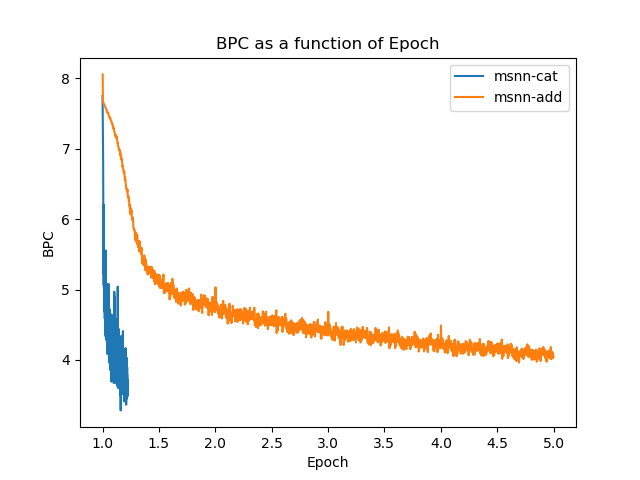
\includegraphics[width=\textwidth]{parts/appendix/reports-gmsnn/docs_esteban-latex/test_reports/comparative-bpc-msnn-det-msnn-cat.png}
	\caption[Performances comparées des stratégies additive et par concaténation]{Performances comparées des stratégies par concaténation (msnn-cat) et additive (msnn-add). Le temps de calcul alloué est identique. Avec la concaténation on entraîne le modèle sur 1/4 des données, avec l'addition on l'entraîne 5 fois sur l'ensemble des données. Avec la concaténation, on obtient une BPC de 3.5, alors qu'on obtient une BPC de 4 avec l'addition.}\label{fig:addcat}
\end{figure} % new

\subsubsection{Sauvegarde, interruption et reprise de l'entraînement}
Une fonctionnalité s'est très vite détachée comme essentielle~: la sauvegarde du \gls{model} et la reprise de l'entraînement.

En effet, avec des entraînements très lents et donc longs, il était nécessaire de pouvoir suspendre l'entraînement affin de répartir le temps de calcul sur plusieurs session de plusieurs heures. De plus, les sauvegardes permettent de conserver le modèle une fois entraîné.

Le système implémenté permet d'effectuer cycliquement des sauvegarde du modèle ainsi que de l'état de l'entraînement, permettant ainsi une reprise en l'état de l'entraînement.

Pour la réalisation du système, le principal obstacle à été le malfonctionnement initial des outils fournis par \gls{pytorch}.
Cela à poussé à la conception d'un système de sauvegarde personnalisé mais malheureusement assez complexe.
Cependant, la mise-à-jour majeure de la librairie qui c'est déroulé à point nommé à résolu le problème, et c'est avec les outils de \gls{pytorch} que le système de sauvegarde à été implémenté.

Voir l'annexe \ref{subsec:save} pour un rapport contenant plus de détail sur le système de sauvegarde. % new
\subsubsection{Tentatives d'optimisations, fuites mémoires et lenteur de l'entraînement}\label{subsec:optimem}

Les optimisations tentées par la suite ont révélé des fuites mémoires et mis en avant une lenteur excessive de l'apprentissage.

Les optimisations en questions ont été mises en suspens le temps de la résolution de ces deux problèmes.
Ces optimisations sont:
\begin{itemize}
	\item l'utilisation de \glspl{batch} simultanés (voir \autoref{subsec:optibatch})~; 
	\item l'augmentation du nombre de \glspl{parameter} du \gls{model} (voir \autoref{subsec:optiparam})~;
\end{itemize}

%\hspace{1em}
\paragraph{Consommation de mémoire et de temps de calcul accrue}
Un effet direct de ces optimisations est l'augmentation de la consommation mémoire.

Cette consommation accrue à causé le plantage de plusieurs tests, révélant la présence de fuites mémoires critiques.
Un ralentissement progressif de l'entraînement à aussi été découvert pendant l'analyse des plantages. % TODO reformuler
Le plus surprenant a été la corrélation forte découverte entre le temps de calcul et la consommation de mémoire.

Un premier correctif à fourni une amélioration notable mais insuffisante.
Il remplaçait le \gls{lstm} de chaque couche (voir \autoref{def:lstm_2}) par un \gls{rnn} basique, moins gourmand. %TODO parler de la redondance 

\paragraph{Estimation de la consommation normale du modèle}
La première étape, qui est détaillée dans l'annexe \ref{subsec:memuse}, à été d'estimer l'usage normal de la mémoire sans fuite, et d'isoler les \glspl{parameter} qui ont le plus d'impact sur la consommation mémoire.
Cela à confirmé que l'explosion de la consommation n'était pas du à l'architecture en elle même, et qu'il s'agissait bien d'une anomalie.

\paragraph{Résolution des fuites}
L'analyse et la résolution des fuites mémoires s'est révélée ardue. Si quelques fuites mineures ont été simple à détecter et réparer, la principale fuite était due à une spécificité non documenté de \gls{pytorch}.

En effet, \gls{pytorch} utilise la \gls{automatic differentiation} pour mettre à jour les \gls{weight} du \gls{nn}.
Pour cela, \gls{pytorch} à besoin de connaître la suite d'opérations et l'implication des différents \glspl{parameter} du \gls{model} et se base sur un \og graphe de computation\fg{}.
C'est la façon dont est gérée ce graphe, couplée aux spécificités de l'architecture \gls{gmsnn} qui est la cause de la principale fuite mémoire.

L'annexe \ref{subsec:memleak} contient une des tentatives de résolution du problème.

% TODO parler de la perf bonasse

\paragraph{Conclusion}
Le problème de la fuite mémoire à été résolu, et avec lui celui de la lenteur de l'entraînement.
On peut déplorer de ne pas avoir analysé plus avant cet étrange lien entre la mémoire et le temps d'entraînement.
Cependant, la résolution des fuites mémoires et de la lenteur de l'entraînement était l'objectif principal de cette étape, et l'optimisation du \gls{module_gmsnn} à pu reprendre. % opti
\subsubsection{Entraînement par exemples simultanés ; \Glsentrytext{batch}} \label{subsec:optibatch}
Une fois le problème des fuites mémoires résolu, la première optimisation mise en place est l'utilisation de \glspl{batch} parallèles.

\paragraph{\gls{batch}}
Un \gls{batch} (anglais pour lot), est un groupe d'exemples successifs.

Le découpage des données en \glspl{batch} permet de répartir l'apprentissage tout au long de l'étude des données.
Cela permet d'atteindre de meilleurs performances.

Il s'agit d'une optimisation rependue pour l'entraînement de \glspl{nn}. % TODO ajouter sources
Elle est souvent couplée à un entraînement simultané sur plusieurs \glspl{batch}.

\paragraph{\Glspl{batch} parallèles}
Un entraînement par \glspl{batch} parallèles permet de calculer le résultat de plusieurs exemples simultanément.
On calcule ensuite la différence de chaque résultat avec le résultat attendu correspondant.
Enfin, on met à jours le \gls{model} en fonction de l'ensemble des exemples.
Au final, les calculs des résultat sont parallélisé, et le coût de la mise à jour est mis en commun entre plusieurs exemples.

Cela permet de réduire drastiquement le temps de calcul et d'améliorer la qualité de l'entraînement, au prix d'une plus grande utilisation de la mémoire.

\paragraph{Conflit entre les \glspl{batch} parallèles et l'architecture \gls{gmsnn}}
Cependant, le découpage en \glspl{batch} pose un problème majeur avec l'architecture \gls{gmsnn}~: elle est basée sur la continuité des exemples fournis, et l'utilisation de \glspl{batch} brise la continuité en introduisant un parallélisme.

Une analyse approfondie à permit d'établir une méthode pour contourner et compenser la majorités des aspect du problème.

Voir le rapport de l'annexe \ref{subsec:batch} pour les détails de l'analyse des problèmes théoriques de l'utilisation de \glspl{batch} avec l'architecture \gls{gmsnn}.

Voir l'annexe \ref{subsec:memuse} pour les détails sur l'impact de la taille des \glspl{batch} et du nombre de \glspl{batch} sur la consommation mémoire.

Voir les annexes\ref{subsec:batch_1}, \ref{subsec:batch_2}, \ref{subsec:batch_3} et \ref{subsec:batch_4} pour les rapports des tests sur la rotation des \glspl{batch}.

\paragraph{Conclusion}
Les problèmes liés à l'utilisation de \glspl{batch} ont été en majorité résolus ou écartés. Après consultation avec notre maître de stage, nous avons décidé d'utiliser l'entraînement par \glspl{batch} malgré les problèmes restants. % new
%nouvelle tentative augmenter params
%aucun impact probant malgré tentative variées
\subsubsection{Augmentation du nombre de paramètres}\label{subsec:optiparam}
Les \glspl{parameter}, ou \glspl{weight}, du modèle sont des valeurs qui varient au long de l'entraînement du \gls{model}. On peut dire que ce sont ces valeurs qui \og apprennent\fg{}.

Le fait d'augmenter ces \glspl{parameter} augmente la qualité de l'apprentissage, et la précision du modèle appris. Mais cela se fait au coût d'un volume plus important du \gls{model}, et d'une augmentation des calculs nécessaires pour utiliser et entraîner le \gls{model}. Cela se manifeste par un entraînement plus lent et une consommation mémoire plus élevée.

Cependant, grâce aux optimisations mises en place durant la résolution des fuites mémoires (voir \autoref{subsec:optimem}), ces coûts ne sont plus dramatiques.

Il existe plusieurs façon de mettre en place cette optimisation~:
\begin{itemize}
	\item augmenter le nombre de neurones par couches~;
	\item augmenter le nombre de couches dans le \glspl{rnn} qui compose chaque \og échelle\fg{}.
\end{itemize}

\paragraph{Conclusion}
Ces deux pratiques ont été testées, et aucune n'apporte d'amélioration de qualité de l'apprentissage, tout en multipliant le temps d'entraînement.
En résumé, ces améliorations apportent des coûts supplémentaires sans aucun bénéfices. % opti
% dernière opti
% algo type EM
% légère amélioration tps de calcul -> graphe
% pas d'améliorattion de perf ->
% révèle pb majeur: seule la première couche semble apprendre -> à priori 90% de l'info est niveau morphologique et syntaxique
\subsubsection{Augmentation du nombre de paramètres}\label{subsec:optilbl}
La dernière optimisation mise en place est un nouvel algorithme d'entraînement.

Cet algorithme est une implémentation naïve d'un entraînement couche par couche appliqué à l'architecture \gls{gmsnn}. Cette algorithme s'apparente aux algorithmes HM \autocite{hm}.

L'intuition à l'origine de l'algorithme est~:
il semble que pour apprendre des représentations de haut niveau, le modèle doit en premier lieu apprendre les représentations de bas niveau~;
en effet, sans mots, il est difficile de faire des phrases cohérentes.

Cela sous-entend que les échelles les plus proches des données doivent apprendre avant que les échelles supérieures puisse apprendre.
Aussi, il semble inutile d'augmenter la charge de l'algorithme d'entraînement en entraînant des couches qui n'apprennent pas.

Le fonctionnent général de cette algorithme est d'entraîner successivement, une à une, les échelles du \gls{model} en commençant par celle la plus proche des données.

Le fonctionnement détaillé de l'algorithme est disponible dans l'annexe \ref{subsec:lbl}.

\paragraph{Performances}
Les performances de l'algorithme sont disponible dans le rapport dans l'annexe \ref{subsec:test_perf}.

L'algorithme remplis sa fonction d'alléger la charge calculatoire. En effet, on à une réduction notable du temps nécessaire pour l'entraînement. % TODO parler de temps constant

De plus, il n'y à aucune variation notable de la qualité de l'entraînement.

%\paragraph{Seule la première couche du modèle semble apprendre}
Justement, comme seule une échelle apprend, on pourrait s'attendre à une baisse des performances.% TODO dire pourquoi.

Comme le \gls{model} muni d'une seule échelle apprend aussi bien que le \gls{model} multi-échelles, cela remet en question l'utilité de l'architecture \gls{gmsnn} et de ses échelles multiples.

\paragraph{Conclusion}
 % new/opti

\subsubsection{Conclusion}
Cette partie du \gls{project_gmsnn} à permit d'améliorer notablement les performances du \gls{model}, tout en réduisant drastiquement le coût d'entraînement.% ccl plus pb mémoire & tps, opti z'oignons (XD) même, 5 min c'est balèze

De plus, l'algorithme présenté \autoref{subsec:optilbl} à démontré une faiblesse majeure de l'architecture \gls{gmsnn}.

On peut aussi noter la mise-à-jour majeure de \gls{pytorch}, qui en plus de résoudre certains dysfonctionnements à nécessité le remaniement d'une partie de la base de code.
 % Optimisation et amélioration du nouveau modèle
\subsection{Production des exemples et découverte du problème d'encodage}
Une fois le modèle fonctionnel, une partie importante de la compréhension et de l'évaluation du modèle est la production d'exemple.

Nous avons retardé cette étape principalement à cause des problèmes de mémoire.

Le principe de cette étape est d'utiliser notre \gls{lm} pour produire du langage, afin d'avoir une idée plus concrète qu'un score de la performance du modèle.

\subsubsection{Exemples}
Voici quelques exemples produits par le modèle. 
La version du modèle choisie est celle avec le meilleur score, parmi celle enregistrées.

Age du modèle~: 465 époques.

Score BPC du modèle~: 1.839.

Pour comparaison, le modèle \gls{soa} avait un score BPC de 1.255 en 50 époques.

Pour rappel, les données sont issues d'une version filtrée de Wikipédia en anglais.

%longstring
\begin{lstlisting}[caption={Exemple 1~: une suite de caractères à priori incompréhensibles.},label=gmsnn_ex1]
YeoMMDF|Ph#elementat[[Damous]]thatureoftenusevoirbeexpounderstatesandanumberofhisworkformembersothan novelwasmethecebylementorfromthelastPreenancenoldWarInstartedbythe Philosophy''theTayita(amsmethouspeopleamingshelebelobesinthesatietheuniversalistscientis educationof[[Lakingforts]].
\end{lstlisting}

%good
\begin{lstlisting}[caption={Exemple 2~: des termes balisé comme dans le corpus d'origine, les crochets ouverts sont refermés.},label=gmsnn_ex2]
+EDrFuergCases,areinlesssuchasthesthealterplains.
*In[[Stefapes]]
*[[AcademyAwards===

ANASA)asLASCIIRunder,andas.MatthebusipenclearsandpresidenthaveaquelfuelsifthesearchfromAwarerLievol ofany30020.

It''[[Anim]]
*[[UnitedStates|raphicsiteDirection]]

Theplant-gainheditsreturnedtoaseethewarinsteast&quot;Oneofthe[ectlywouldnotbytheIntegrationscapianland](ora''[[schology]]
|published:
\end{lstlisting}

%longstring + tags
\begin{lstlisting}[caption={Exemple 3~: des termes balisé comme dans l'exemple 2, et une autre suite de carractères.},label=gmsnn_ex3]
60447-toNewHarry}}
Thenmainst.Rand'sintereststhe&quot;toinpassingtheEarth''s(''[[par]].

:'''maimals,anackreloquedoutwidthofgrawwithluteframedapproyingtoundernverby[[hebesination]]of&lt;/smalkan,instablishedacondorttodevelopedframesbeforestatedwinkingaroundinrational hicarefartoredonaftercanbeagainsthatgroupswouldnear,notwhatwasthatisstillastructionCenter,toDagnythat

On[[teleofAirëejã]]
[[cy:Alaska]]
[[no:Arni-Anchorages]]
\end{lstlisting}

\subsubsection{Manque d'espaces}
Parmi ces exemples, on remarque immédiatement le manque d'espace.

La source de ce phénomène n'est autre qu'un problème dans le corpus source.
La version pré-traitée de ce corpus ne contenait aucun espace, donc le \gls{model} à appris une langue dans laquelle l'espace n'existe pas.

C'est un problème majeur, qui à probablement eu un impact élevé sur les performances du modèle. En effet, en anglais comme dans beaucoup de langues occidentales, l'espace est un élément fondamental dans la structuration du langage écrit. Le \gls{model} à ainsi apprit une langue moins structurée, donc plus difficile à apprendre, que l'anglais.

\subsubsection{Quelque éléments qui ressortent}
Cependant, si on regarde plus en détail les exemples produits, des structures apparaissent. 

Si on prend \lstinline!*[[UnitedStates|raphicsiteDirection]]! de l'exemple 2 (\autoref{gmsnn_ex2}, ligne 8) ou 
\lstinline![[cy:Alaska]]! et \lstinline![[no:Arni-Anchorages]]! de l'exemple 2 (\autoref{gmsnn_ex2}, lignes 7 et 8), on a des doubles crochets, qui sont correctement ouverts puis fermés. On remarque aussi la présence de séparateurs (\lstinline!:! et \lstinline!|!).

Ces structure sont similaire aux annotations présentes dans le code Wikipédia.

Enfin, malgré l'absence d'espaces, on discerne de nombreux mots~:
\begin{itemize}
\item la suite de mots \lstinline!statesandanumberofhisworkformembersothannovelwasmethe! qui ne contient en fait que des mots bien formés en anglais~: \lstinline!states and a number of his work for member so than novel was me the! (\autoref{gmsnn_ex1}, ligne 1);
\item de même pour la suite de mots \lstinline!oldWarInstartedbythePhilosophy!~: \lstinline!old War In started by the Philosophy! (\autoref{gmsnn_ex1}, ligne 1);
\item on trouve aussi des noms propres comme le nom de pays~: \lstinline!UnitedStates! (\autoref{gmsnn_ex2}, ligne 8) et \lstinline!Alaska! (\autoref{gmsnn_ex3}, ligne 7).
\end{itemize}
\section{Analyse des résultats et arrêt du projet}\label{white_flag}
% Durant la periode d'optimisations, j'avais préparé plein de trucs
% Je les ai tous testés: aucun changement de perf, légère opti tps

% Ca + tout "corrompu" par dataset foiré

% + Retour de réunion sur papud
% => arret du projet et passage sur papud
% gmsnn opti, mais pas assez performant

\subsection{Analyse des résultats}
Avec notre maître de stage, nous avons étudié attentivement les résultats des dernières optimisations sur les performances du \gls{model} (voir annexe \ref{subsec:test_perf}). 
Le résultat le plus dérangeant était l'absence d'apprentissage des couche supérieures.

À partir des connaissances de la littérature possédées par notre maître de stage et de ce résultat, nous avons conclu que 90\% de l'information nécessaire est apprise par la première échelle du modèle. Les autres échelles ne font qu'améliorer ce résultat, et sont peu utiles tant que la première échelle n'est pas complètement entraînée.

À cela s'ajoute la disparition des espaces du corpus, qui nécessiterait non seulement de remanier une partie du code tenue pour acquise, mais aussi de refaire la plupart des tests effectués.

\subsection{Conclusions de l'analyse}
La conclusion à laquelle nous sommes arrivés est qu'il aurait fallu recommencer le développement avec un système de gestion des données maîtrisé et changer le processus de développement du modèle.

La première étape aurait été de développer un modèle simple, avec une seule échelle, et de le pousser au maximum de ses capacités. Seulement à ce moment là nous aurions pu l'augmenter d'autres échelles.

Il aurait aussi été intéressant de revoir l'architecture pour utiliser un modèle sans récurrences.

Cette conclusion impliquait de recommencer le projet, ou à défaut de le remanier en grande partie.

\subsection{Arrêt du projet et début du projet suivant}
Au moment de cette analyse, notre maître de stage revenait d'une réunion décisive sur le \gls{project_papud}.

Celle-ci avait permis de définir les objectifs du \glsfirst{project_papud} (voir \autoref{ch:project_papud}), qui ont été influencés par nos conclusions.

La nécessité de recommencer le \gls{project_gmsnn}, couplée à l'opportunité de mettre les conclusions et les compétences acquises en pratique dans un projet à grande échelle, nous ont mené à interrompre \gls{project_gmsnn} pour consacrer la fin du stage au \gls{project_papud}.

C'est d'un commun accord avec notre maître de stage que nous avons décidé de basculer sur le \gls{project_papud}.
\subsection{Conclusions}
% TODO production des résultats -> nospace
Ce projet nous à permit d'implémenter une architecture innovante de \gls{nn}, à partir d'un modèle état de l'art.

% ccl plus pb mémoire & tps, opti z'oignons (XD) même, 5 min c'est balèze
C'est la première pierre de l'édifice qu'est le \gls{gmsnn}.
mise en œuvre de l'architecture proposée. La dernière étape est d'améliorer les performances du modèle, et de l'optimiser.
Cette partie du \gls{project_gmsnn} à permit d'améliorer notablement les performances du \gls{model}, tout en réduisant drastiquement le coût d'entraînement.

De plus, l'algorithme présenté \autoref{subsec:optilbl} à démontré une faiblesse majeure de l'architecture \gls{gmsnn}.
La réalisation de ce projet nous à permit d'approfondir largement nos connaissances en \gls{dl}. 


\section{\Glsentrytext{project_papud}}
\subsection{Recherche documentaire} % lib, tutos, concepts
\subsection{Ré-implémentation simplifiée du modèle \glsentrytext{soa}} % reprise sur de l'existant, découverte de la lib
\subsection{Implémentation du nouveau modèle basique} % reprise sur de l'existant
\subsection{Optimisation et amélioration du nouveau modèle}
\subsection{Conclusions}


\section{Documentation}


%Il est aisé d'insérer du code dans un rapport. Il suffit de définir le langage, la légende à afficher et enfin un Label pour pouvoir y faire référence. Le résultat est donnée dans le listing \ref{lst:premierExemple}. Il est également possible de changer les couleurs, pour cela il faut éditer le lstset dans la classe tnreport.cls.

%\begin{lstlisting}[language=c++, caption={Premier Exemple}, label={lst:premierExemple}]
%void CEquation::IniParser()
%{
%if (!pP){ //if not already initialized...
%pP = new mu::Parser;
%
%pP->DefineOprt("%", CEquation::Mod, 6); //deprecated
%pP->DefineFun("mod", &CEquation::Mod, false);
%pP->DefineOprt("&", AND, 1); //DEPRECATED
%pP->DefineOprt("and", AND, 1);
%pP->DefineOprt("|", OR, 1); //DEPRECATED
%pP->DefineOprt("or", OR, 1);
%pP->DefineOprt("xor", XOR, 1);
%pP->DefineInfixOprt("!", NOT);
%pP->DefineFun("floor", &CEquation::Floor, false);
%pP->DefineFun("ceil", &CEquation::Ceil, false);
%pP->DefineFun("abs", &CEquation::Abs, false);
%pP->DefineFun("rand", &CEquation::Rand, false);
%pP->DefineFun("tex", &CEquation::Tex, false);
%
%pP->DefineVar("x", &XVar);
%pP->DefineVar("y", &YVar);
%pP->DefineVar("z", &ZVar);
%}
%}
%\end{lstlisting}
%\clearpage
%Il est également possible d'afficher du code directement depuis un fichier source, le résultat de cette opération est visible dans le listing \ref{lst:fromSrc}
%\lstinputlisting[language=c++,caption={Affichage depuis le fichier source},label={lst:fromSrc}]{figures/sourceCode.cpp}